%TODO alles zusammenfügen und in ein Dokument mit SRCREPORT und Chapters (gemäss Ordnerstruktur)
\documentclass[11pt,a4paper, parskip,ngerman] {report} 


%Preamble for the Document for reuse and the last Document
\author{\authors}
\date{\today{}}
\title{\arbeit}
\usepackage[T1]{fontenc} % Font family encoding: 8 Bit
\usepackage[utf8]{inputenc} % Encoding in the created document: UTF-8
\usepackage[sfdefault]{FiraSans} % Font family
\renewcommand*\oldstylenums[1]{{\firaoldstyle #1}}
\usepackage[babel]{microtype} % Automatische Grauwertverbesserung
\usepackage[ngerman]{babel}
\usepackage[automark]{scrpage2}
\usepackage[colorlinks = true,
linkcolor = black]{hyperref}
\usepackage{color}
\usepackage[normalem]{ulem}
\usepackage{scrpage2}
\usepackage{graphicx}
\usepackage{tabularx}
\usepackage{textcomp}

\usepackage{framed}
\usepackage{geometry}
\usepackage{minutes}
\usepackage{lscape}
\usepackage[table]{xcolor}
\usepackage{multicol}
\usepackage{longtable,tabu}

\usepackage[style=numeric,,sorting=none,backend=bibtex]{biblatex}
\addbibresource{./SDDC.bib}
\usepackage{titlesec}
\usepackage[printonlyused] {acronym}
\titleformat{\chapter}{\normalfont\huge\bf}{\thechapter}{20pt}{\huge\bf}
\pagestyle{plain}
\usepackage{caption}
\usepackage{subcaption}
\usepackage{pdfpages}

\usepackage{tikz}
\usepackage{pgf-pie}
\usetikzlibrary{positioning,shadings}
\usetikzlibrary{arrows}
\usepackage{pbox}
\definecolor{logocolor}{RGB}{6,103,236}
%Code Listing 
\usepackage{color}
\usepackage{listings}

\definecolor{mygreen}{rgb}{0,0.6,0}
\definecolor{mygray}{rgb}{0.5,0.5,0.5}
\definecolor{mymauve}{rgb}{0.58,0,0.82}
%Standard
\lstset{ %
  backgroundcolor=\color{white},  
  basicstyle=\footnotesize,        
  breakatwhitespace=false,         
  breaklines=true,               
  captionpos=b,                  
  commentstyle=\color{mygreen},    
  deletekeywords={...},            
  escapeinside={\%*}{*)},          
  extendedchars=true,           
  frame=single,	                   
  keepspaces=true,                 
  keywordstyle=\color{blue},      
  language=Octave,                 
  otherkeywords={*,...},           
  numbers=none,                    
  rulecolor=\color{black},         
  showspaces=false,               
  showstringspaces=false,          
  showtabs=false,                
  stepnumber=2,                    
  stringstyle=\color{mymauve},     
  tabsize=2,	                   
  title=\lstname             
}

%Java
\definecolor{dkgreen}{rgb}{0,0.6,0}
\definecolor{gray}{rgb}{0.5,0.5,0.5}
\definecolor{mauve}{rgb}{0.58,0,0.82}
\definecolor{light-gray}{gray}{0.25}

\lstdefinestyle{java}{
  language=Java,
  aboveskip=3mm,
  belowskip=3mm,
  showstringspaces=false,
  columns=flexible,
  basicstyle={\footnotesize\ttfamily},
  numberstyle={\tiny},
  numbers=none,
  keywordstyle=\color{blue},
  commentstyle=\color{dkgreen},
  stringstyle=\color{mauve},
  breaklines=true,
  breakatwhitespace=true,
  tabsize=3
}



%JSON Styles
\colorlet{punct}{red!60!black}
\definecolor{background}{HTML}{EEEEEE}
\definecolor{delim}{RGB}{20,105,176}
\colorlet{numb}{magenta!60!black}

\lstdefinelanguage{json}{
    stepnumber=1,
    breaklines=true,
    literate=
     *{0}{{{\color{numb}0}}}{1}
      {1}{{{\color{numb}1}}}{1}
      {2}{{{\color{numb}2}}}{1}
      {3}{{{\color{numb}3}}}{1}
      {4}{{{\color{numb}4}}}{1}
      {5}{{{\color{numb}5}}}{1}
      {6}{{{\color{numb}6}}}{1}
      {7}{{{\color{numb}7}}}{1}
      {8}{{{\color{numb}8}}}{1}
      {9}{{{\color{numb}9}}}{1}
      {:}{{{\color{punct}{:}}}}{1}
      {,}{{{\color{punct}{,}}}}{1}
      {\{}{{{\color{delim}{\{}}}}{1}
      {\}}{{{\color{delim}{\}}}}}{1}
      {[}{{{\color{delim}{[}}}}{1}
      {]}{{{\color{delim}{]}}}}{1},
}

%XML
\definecolor{forestgreen}{RGB}{34,139,34}
\definecolor{orangered}{RGB}{239,134,64}
\definecolor{darkblue}{rgb}{0.0,0.0,0.6}
\definecolor{gray}{rgb}{0.4,0.4,0.4}

\lstdefinestyle{XML} {
    language=XML,
    extendedchars=true, 
    breaklines=true,
    breakatwhitespace=true,
    emph={},
    emphstyle=\color{red},
    basicstyle=\ttfamily,
    columns=fullflexible,
    commentstyle=\color{gray}\upshape,
    morestring=[b]",
    morecomment=[s]{<?}{?>},
    morecomment=[s][\color{forestgreen}]{<!--}{-->},
    keywordstyle=\color{orangered},
    stringstyle=\ttfamily\color{black}\normalfont,
    tagstyle=\color{darkblue}\bf,
    morekeywords={attribute,xmlns,version,type,release},
    otherkeywords={attribute=, xmlns=},
}


%Bash
\lstdefinestyle{Bash}
{
 language=bash,
 frame=single,
  showstringspaces=false,
  commentstyle=\color{green},
  keywordstyle=\color{blue}
}

\titlespacing*{\subsection}
{0pt}{5.5ex plus 1ex minus .2ex}{4.3ex plus .2ex}

\usepackage{glossaries}
\makeglossaries
%Definition of frequently used Texts
\newcommand{\advisor}
	{Urs Baumann}
\newcommand{\advisorprof}
	{Prof. Beat Stettler}
\newcommand{\contraprof}
	{TBA}
\newcommand{\expert}
	{TBA}
\newcommand{\authors}
	{Silvan Adrian, Fabian Binna}
\newcommand{\place}
	{Hochschule für Technik Rapperswil \\ Institute for Networked Solutions}
\newcommand{\ins}
	{Institute for Networked Solutions}
\newcommand{\timeperiod}
	{Herbstsemester 2015}
\newcommand{\titel}
	{SDDC \\ Software Defined Data Center}
\newcommand{\arbeit}
	{Semesterarbeit }	


\begin{document}
%Inputs Config
%%Definition of frequently used Texts
\newcommand{\advisor}
	{Urs Baumann}
\newcommand{\advisorprof}
	{Prof. Beat Stettler}
\newcommand{\contraprof}
	{TBA}
\newcommand{\expert}
	{TBA}
\newcommand{\authors}
	{Silvan Adrian, Fabian Binna}
\newcommand{\place}
	{Hochschule für Technik Rapperswil \\ Institute for Networked Solutions}
\newcommand{\ins}
	{Institute for Networked Solutions}
\newcommand{\timeperiod}
	{Herbstsemester 2015}
\newcommand{\titel}
	{SDDC \\ Software Defined Data Center}
\newcommand{\arbeit}
	{Semesterarbeit }	

%\documentclass[11pt,a4paper, parskip,ngerman] {report} 


%Preamble for the Document for reuse and the last Document
\author{\authors}
\date{\today{}}
\title{\arbeit}
\usepackage[T1]{fontenc} % Font family encoding: 8 Bit
\usepackage[utf8]{inputenc} % Encoding in the created document: UTF-8
\usepackage[sfdefault]{FiraSans} % Font family
\renewcommand*\oldstylenums[1]{{\firaoldstyle #1}}
\usepackage[babel]{microtype} % Automatische Grauwertverbesserung
\usepackage[ngerman]{babel}
\usepackage[automark]{scrpage2}
\usepackage[colorlinks = true,
linkcolor = black]{hyperref}
\usepackage{color}
\usepackage[normalem]{ulem}
\usepackage{scrpage2}
\usepackage{graphicx}
\usepackage{tabularx}
\usepackage{textcomp}

\usepackage{framed}
\usepackage{geometry}
\usepackage{minutes}
\usepackage{lscape}
\usepackage[table]{xcolor}
\usepackage{multicol}
\usepackage{longtable,tabu}

\usepackage[style=numeric,,sorting=none,backend=bibtex]{biblatex}
\addbibresource{./SDDC.bib}
\usepackage{titlesec}
\usepackage[printonlyused] {acronym}
\titleformat{\chapter}{\normalfont\huge\bf}{\thechapter}{20pt}{\huge\bf}
\pagestyle{plain}
\usepackage{caption}
\usepackage{subcaption}
\usepackage{pdfpages}

\usepackage{tikz}
\usepackage{pgf-pie}
\usetikzlibrary{positioning,shadings}
\usetikzlibrary{arrows}
\usepackage{pbox}
\definecolor{logocolor}{RGB}{6,103,236}
%Code Listing 
\usepackage{color}
\usepackage{listings}

\definecolor{mygreen}{rgb}{0,0.6,0}
\definecolor{mygray}{rgb}{0.5,0.5,0.5}
\definecolor{mymauve}{rgb}{0.58,0,0.82}
%Standard
\lstset{ %
  backgroundcolor=\color{white},  
  basicstyle=\footnotesize,        
  breakatwhitespace=false,         
  breaklines=true,               
  captionpos=b,                  
  commentstyle=\color{mygreen},    
  deletekeywords={...},            
  escapeinside={\%*}{*)},          
  extendedchars=true,           
  frame=single,	                   
  keepspaces=true,                 
  keywordstyle=\color{blue},      
  language=Octave,                 
  otherkeywords={*,...},           
  numbers=none,                    
  rulecolor=\color{black},         
  showspaces=false,               
  showstringspaces=false,          
  showtabs=false,                
  stepnumber=2,                    
  stringstyle=\color{mymauve},     
  tabsize=2,	                   
  title=\lstname             
}

%Java
\definecolor{dkgreen}{rgb}{0,0.6,0}
\definecolor{gray}{rgb}{0.5,0.5,0.5}
\definecolor{mauve}{rgb}{0.58,0,0.82}
\definecolor{light-gray}{gray}{0.25}

\lstdefinestyle{java}{
  language=Java,
  aboveskip=3mm,
  belowskip=3mm,
  showstringspaces=false,
  columns=flexible,
  basicstyle={\footnotesize\ttfamily},
  numberstyle={\tiny},
  numbers=none,
  keywordstyle=\color{blue},
  commentstyle=\color{dkgreen},
  stringstyle=\color{mauve},
  breaklines=true,
  breakatwhitespace=true,
  tabsize=3
}



%JSON Styles
\colorlet{punct}{red!60!black}
\definecolor{background}{HTML}{EEEEEE}
\definecolor{delim}{RGB}{20,105,176}
\colorlet{numb}{magenta!60!black}

\lstdefinelanguage{json}{
    stepnumber=1,
    breaklines=true,
    literate=
     *{0}{{{\color{numb}0}}}{1}
      {1}{{{\color{numb}1}}}{1}
      {2}{{{\color{numb}2}}}{1}
      {3}{{{\color{numb}3}}}{1}
      {4}{{{\color{numb}4}}}{1}
      {5}{{{\color{numb}5}}}{1}
      {6}{{{\color{numb}6}}}{1}
      {7}{{{\color{numb}7}}}{1}
      {8}{{{\color{numb}8}}}{1}
      {9}{{{\color{numb}9}}}{1}
      {:}{{{\color{punct}{:}}}}{1}
      {,}{{{\color{punct}{,}}}}{1}
      {\{}{{{\color{delim}{\{}}}}{1}
      {\}}{{{\color{delim}{\}}}}}{1}
      {[}{{{\color{delim}{[}}}}{1}
      {]}{{{\color{delim}{]}}}}{1},
}

%XML
\definecolor{forestgreen}{RGB}{34,139,34}
\definecolor{orangered}{RGB}{239,134,64}
\definecolor{darkblue}{rgb}{0.0,0.0,0.6}
\definecolor{gray}{rgb}{0.4,0.4,0.4}

\lstdefinestyle{XML} {
    language=XML,
    extendedchars=true, 
    breaklines=true,
    breakatwhitespace=true,
    emph={},
    emphstyle=\color{red},
    basicstyle=\ttfamily,
    columns=fullflexible,
    commentstyle=\color{gray}\upshape,
    morestring=[b]",
    morecomment=[s]{<?}{?>},
    morecomment=[s][\color{forestgreen}]{<!--}{-->},
    keywordstyle=\color{orangered},
    stringstyle=\ttfamily\color{black}\normalfont,
    tagstyle=\color{darkblue}\bf,
    morekeywords={attribute,xmlns,version,type,release},
    otherkeywords={attribute=, xmlns=},
}


%Bash
\lstdefinestyle{Bash}
{
 language=bash,
 frame=single,
  showstringspaces=false,
  commentstyle=\color{green},
  keywordstyle=\color{blue}
}

\titlespacing*{\subsection}
{0pt}{5.5ex plus 1ex minus .2ex}{4.3ex plus .2ex}

\usepackage{glossaries}
\makeglossaries


%\begin{document}
\newgeometry{left=2.25cm, right=2.25cm, top=2.25cm, bottom=2.25cm} % new
% margins



\begin{titlepage}
%TODO: set logo position exactly.
\begin{center}
\begin{minipage}[t]{0.45\textwidth}
    
\includegraphics[width=\textwidth]{./22_Grafiken/01_Logo/hsrLogo}
\end{minipage}
\hspace{\fill} % horizontal space
\begin{minipage}[t]{0.45\textwidth}
    \vspace{-2.9cm}
    
\includegraphics[width=\textwidth]{./22_Grafiken/01_Logo/ins} %TODO: more highres logo
\end{minipage}

\end{center}

\vspace{15ex} % vertical space
\begin{center}
	\Huge 
	\begin{framed}
		\textbf{\titel}
	\end{framed}
	
	\vspace{3ex}
	\textbf{\arbeit}
	
	\vspace{1ex}
	\LARGE 
	\place
	
	\vspace{5ex}
	\begin{framed}
		\timeperiod
	\end{framed}
\end{center}

\vspace{11ex}
\begin{tabular}{ll} % Table
	Autoren:         		& \authors	\\
	Betreuender Dozent:		& \advisorprof  	\\
	Betreuer:        		& \advisor    	\\
	Gegenleser:      		& \contraprof  	\\
	Experte:      			& \expert  		\\
	Projektpartner:      	& \ins  		\\
\end{tabular}

\end{titlepage}

\restoregeometry % reset page margins
%\end{document}
\chapter*{Abstract}\addcontentsline{toc}{chapter}{Abstract}

Unter „Software Defined“ versteht man die Zentralisierung der Intelligenz in Kontrollern. Gerade moderne Data Center werden immer häufiger von Software Kontrollern gesteuert, damit die Dynamik der Bereitstellung von neuen Services massiv erhöht werden kann. Ziel ist, die Ressourcen Storage, Network und Compute abstrahiert als skalierbare Pools der „Service Ebene“ zur Verfügung zu stellen.\\
Eine RESTful API, die den Umgang mit Services, die wiederum Pakete von Ressourcen darstellen, sorgt für einen zentralen Punkt, an den diverse Systeme und Business Applikationen anknüpfen können. Damit die breite Auswahl von Libraries und Produkten in einem Data Center angesprochen werden kann, verwaltet eine generische API die Kontroller und ermöglicht den abstrakten Umgang mit Ressourcen. Die beiden abstrakten Ebenen, RESTful API und generische API, werden mit einem Workflow verbunden. Der Workflow kümmert sich um den zeitlich korrekten Ablauf der Instantiierung. Die Software kann als Webservice in einem Docker Container ausgerollt werden und benötigt danach nur noch eine Konfiguration der generischen API und der Kontroller.

\chapter*{Erklärung der Eigenständigkeit}

Ich erkläre hiermit,

\begin{itemize}
  \item dass ich die vorliegende Arbeit selber und ohne fremde Hilfe durchgeführt habe, ausser derjenigen, 
  welche explizit in der Aufgabenstellung erwähnt ist oder mit dem Betreuer schriftlich vereinbart wurde,
  \item dass ich sämtliche verwendeten Quellen erwähnt und gemäss gängigen 
  wissenschaftlichen Zitierregeln korrekt angegeben habe.
  \item das ich keine durch Copyright geschützten Materialien (z.B. Bilder) 
  in dieser Arbeit in unerlaubter Weise genutzt habe. 
\end{itemize}

\textbf{Ort, Datum:}

Raperswil-Jona, \today


\textbf{Name, Unterschrift}



\includegraphics[width=0.25\textwidth]{01_Einleitung/images/unterschrift-sadrian}

Silvan Adrian

\newpage
Ich erkläre hiermit,

\begin{itemize}
  \item dass ich die vorliegende Arbeit selber und ohne fremde Hilfe durchgeführt habe, ausser derjenigen, 
  welche explizit in der Aufgabenstellung erwähnt ist oder mit dem Betreuer schriftlich vereinbart wurde,
  \item dass ich sämtliche verwendeten Quellen erwähnt und gemäss gängigen 
  wissenschaftlichen Zitierregeln korrekt angegeben habe.
  \item das ich keine durch Copyright geschützten Materialien (z.B. Bilder) 
  in dieser Arbeit in unerlaubter Weise genutzt habe. 
\end{itemize}

\textbf{Ort, Datum:}

Raperswil-Jona, \today


\textbf{Name, Unterschrift}



Fabian Binna
\tableofcontents



\chapter{Aufgabenstellung}

Unter ``Software Defined'' versteht man die Zentralisierung der Intelligenz in Kontrollern. 
Gerade moderne Data Center werden immer mehr von Software Kontrollern gesteuert, 
damit die Dynamik der Bereitstellung von neuen Services massiv erhöht werden kann. 
So gibt es bereits Kontroller für Storage, Netzwerk und Compute Ressourcen. 
\\ \\
Ziel ist es, die Ressourcen Storage, Network und Compute abstrahiert als skalierbare Pools der 
``Service Ebene'' zu Verfügung zu stellen. Alle modernen Kontroller können über API's 
angesprochen werden, allerdings unterscheiden sich hier die verschiedenen Hersteller zum Teil stark.
\\ \\
Ziel dieser Arbeit ist die Entwicklung einer generischen Middleware/API, um verschiedene Kontroller 
möglichst einfach in Business Applikationen zu integrieren. Nach der Definition einer systemunabhängigen 
Schnittstelle sollen die verschiedenen Kontroller danach als Treiber an die API angehängt werden können. 
Zur Demonstrationszwecken soll eine rudimentäre, ca. 3 Seitige Webpage erstellt werden, welche die erstelle 
API benützt. Dabei soll je mind. ein Storage, Compute und Network Kontroller eingebunden werden.


%Analyse


\subsection{API}
\begin{itemize}
\item Die API sollte auf einem möglichst stabilen Stand sein.
\item Es müssen die wichtigsten Provider zur Verfügung stehen.
\item Die API muss gut dokumentiert sein.
\item Es sollen verschiedene Services angesprochen werden können (Compute, Storage, Network...).
\item Keine grosse Einarbeitung, das heisst die Programmiersprache sollte nicht komplett neu sein.
\end{itemize}

Zudem sind alle Eingenschaften die das Implementieren der Software erleichtern ein 
Pluspunkt. Von Vorteil währen zusätzliche Funktionen wie z.B SSL oder Pricing. 

\subsection{User-Dashboard}
Das User-Dashboard soll eine Möglichkeit für Benutzer bieten, um einzelne Services 
abonnieren zu können.
Dabei soll sowohl \ac{IaaS}, \ac{PaaS} oder \ac{SaaS} abonniert werden können und eine Auswahl 
bieten unter vielen verschiedenen Cloud Anbietern wählen zu können (so generisch wie 
möglich).
Dabei soll der User zwischen einzelnen Angeboten der Anbieter spezifischen 
Services zu wählen bspw.: bei Google Cloud: Cloud DNS, Firewall, Netzwerke etc.
Es kann daher auch sein das nicht alle Anbieter die gleichen Services bieten und 
daher eine Auswahl gegeben werden muss, damit der Benutzer selbst entscheiden 
kann welchen Service er haben will.

\subsubsection{SDDC}
Unser Projekt soll deshalb eine einiges generische Möglichkeit bieten, um 
Service abonnieren zu können und wenn möglich so gut wie alle Cloud Anbieter zu 
unterstützen.
Dies soll möglich werden indem ein Dashboard eine generische API anspricht und 
die API alle Schritte durchführt, die nötig sind für die Erstellung des 
Services.

\subsection{Admin-Dashboard}
Dem Admin soll eine Möglichkeit geboten werden um die Software administrieren zu 
können, z.B.: Benutzerverwaltung oder etwas in der Art.

\input{./03_Analyse/02_API/api-analyse}
\input{./03_Analyse/03_Bitnami/bitnami-analyse}
\documentclass[11pt]{scrartcl}

\title{Use Case Skizzen}
\author{Silvan Adrian \\ Fabian Binna}
\date{\today{}}

\usepackage[ngerman]{babel}
\usepackage[automark]{scrpage2}
\usepackage{hyperref}
\usepackage{color}
\usepackage[normalem]{ulem}
\usepackage{scrpage2}
\usepackage{graphicx}
\usepackage{tabularx}
\graphicspath{ {../22_Grafiken/01_Logo/}{images/}{../../22_Grafiken/01_Logo/} }
\pagestyle{scrheadings}

\clearscrheadfoot
\ihead{
\includegraphics[scale=0.3]{SDDC}}
\ohead{Projekt: SDDC}
\ifoot{Use Case Skizzen}
\cfoot{Version: 1.01}
\ofoot{Datum: \today{}}
\setheadsepline{0.5pt}
\setfootsepline{0.5pt}

\usepackage{ucs}
\usepackage[utf8]{inputenc}
\usepackage[T1]{fontenc}


\begin{document}
\def\arraystretch{1.5}
\begin{titlepage}
\begin{center}
\vspace{10em}

\includegraphics[scale=2]{SDDC}
\vspace{10em}
\end{center}
\begin{center}
\huge {Template}
\end{center}
\begin{center}
\vspace{10em}
\LARGE {Silvan Adrian} \\
\LARGE {Fabian Binna}
\end{center}

\end{titlepage}

\newpage
\section{Änderungshistorie}
\begin{tabularx}{\linewidth}{l l X l}
\textbf{Datum} & \textbf{Version} & \textbf{Änderung}  & \textbf{Autor} \\
\hline
\textbf{25.09.15} & 1.00 & Erstellung des Dokuments & Gruppe \\
\textbf{25.06.15} & 1.01 & Aktoren und Use Cases aus dem Diagramm & Silvan 
Adrian\\
\textbf{27.09.15} & 1.02 & Diagramm eingefügt + Verbesserungen & Silvan Adrian\\
\end{tabularx}

\newpage
\tableofcontents
\newpage
\section{Akteure}
\begin{tabularx}{\linewidth}{X X}
\textbf{Akteur} & \textbf{Ziel}\\
\hline
\textbf{Public User} &
Registrieren
\\
\hline
\textbf{Registered User} & 
\textbf{Wenn User:}

Login

Logout

Service anlegen (Create)

Service Infos lesen (Read)

Service ändern (Update)

Service löschen (Delete)

Benutzerinfos ändern

\textbf{Wenn Admin:}

Benutzer anlegen

Benutzer löschen

Benutzer ändern

Benutzerinfos ändern

\\
\hline
\textbf{Cloud Anbieter} &
Service anlegen (Create)

Service Infos lesen (Read)

Service ändern (Update)

Service löschen (Delete)
\\

\end{tabularx}


\section{Use Case Diagramm}


\includegraphics[width=\textwidth]{UseCase-Skizzen}



\end{document}
\documentclass[11pt]{scrartcl}

\title{User Stories Skizzen}
\author{Silvan Adrian \\ Fabian Binna}
\date{\today{}}

\usepackage[ngerman]{babel}
\usepackage[automark]{scrpage2}
\usepackage[colorlinks = true,
linkcolor = black]{hyperref}
\usepackage{color}
\usepackage[normalem]{ulem}
\usepackage{scrpage2}
\usepackage{graphicx}
\usepackage{tabularx}
\graphicspath{ {../22_Grafiken/01_Logo/}{images/}{../../22_Grafiken/01_Logo/} }
\pagestyle{scrheadings}

\clearscrheadfoot
\ihead{
\includegraphics[scale=0.3]{SDDC}}
\ohead{Projekt: SDDC}
\ifoot{User Stories Skizzen}
\cfoot{Version: 1.02}
\ofoot{Datum: \today{}}
\setheadsepline{0.5pt}
\setfootsepline{0.5pt}

\usepackage{ucs}
\usepackage[utf8]{inputenc}
\usepackage[T1]{fontenc}


\begin{document}
\def\arraystretch{1.5}
\begin{titlepage}
\begin{center}
\vspace{10em}

\includegraphics[scale=2]{SDDC}
\vspace{10em}
\end{center}
\begin{center}
\huge {User Stories Skizzen}
\end{center}
\begin{center}
\vspace{10em}
\LARGE {Silvan Adrian} \\
\LARGE {Fabian Binna}
\end{center}

\end{titlepage}

\newpage
\section{Änderungshistorie}
\begin{tabularx}{\linewidth}{l l X l}
\textbf{Datum} & \textbf{Version} & \textbf{Änderung}  & \textbf{Autor} \\
\hline
\textbf{26.09.15} & 1.00 & Erstellung des Dokuments & Gruppe \\
\textbf{26.09.15} & 1.01 & Einführung + Rollen & Silvan Adrian \\
\textbf{27.09.15} & 1.02 & Ziele + kurze User Stories Skizzen & Silvan Adrian\\
\end{tabularx}

\newpage
\tableofcontents
\newpage
\section{Einführung}

\subsection{Zweck}

Dieses Dokument beinhaltet die ersten Skizzen der User Stories.

\subsection{Gültigkeitsbereich}

Dieses Dokument ist während des ganzen Projekts gültig.


\subsection{Referenzen}
Bitnami-Analyse.pdf\\
Dashboard-Analyse.pdf\\
UseCase-Skizzen.pdf

\section{Rollen}
\subsection{Public User}
Public User sind alle öffentlichen Besucher des Dashboards.

\subsection{Registered User}
Der registrierte Nutzer ist Anwender des Dashboards und verwendet dieses zur 
Aufgabenerleichterung.
Bei dem Nutzer kann es sich um einen System Administrator, DevOps, Operator oder
Software Entwickler handlen, da beim Dashboard für jeden was dabei ist.

\subsection{Admin}
Der Admin ist für die Instandhaltung des Dashboards zuständig und verwaltet die 
User.

\section{Ziele}
Im Umfang soll die Applikation in etwa folgendes bieten:
\begin{itemize}
  \item Registrierung (Mail Adresse/Passwort)
  \item Login
  \item Administrationoberfläche
  \item Benutzerinfos anpassen
  \item Auswahl aus mehreren Cloud Anbieter
  \item mehrere Cloud Accounts hinzufügen
  \item Abonnieren von Services (Compute/Storage/Network)
  \item Unterteilung der Services in Compute/Storage/Network
  \item Übersicht aller zur Verfügung stehenden Services
  \item Management der Services (erstellen/ändern/löschen)
  \item Links zu Loginpanels von Cloud Anbieter
  \item Übersicht über abonnierte Services
  \item Unterstützung Private Cloud (OpenStack,CloudStack, Docker(Deis -> PaaS))
  \item Anbieter spezifische Services anbieten
  \item generische API
  \item Anstehende Kosten anzeigen
  \item Einfaches hinzufügen eines Cloud Accounts (Wizard bieten)
\end{itemize}


\section{Epic}
\begin{itemize}
  \item Service abonnieren (Compute/Storage/Network)
\end{itemize}

\section{User Stories}

\subsection{Public User}
\begin{itemize}
  \item Als Public User möchte ich mich registrieren können
  \item Als Public User möchte ich mich auf Dashboard verbinden, um einloggen zu 
  können
\end{itemize}
\subsection{Registered User}
\begin{itemize}
  \item Als registered User möchte ich mich einloggen können
  \item Als registered User möchte ich eine Übersicht aller angebotenen Cloud 
  Anbieter sehen
  \item Als registered User möchte ich Zugriff auf meine Accountinfos
  \item Als registered User möchte ich meine Accountinfos anpassen können
  \item Als registered User möchte ich ein Cloud Anbieter auswählen können, um 
  auf die Übersicht der Offerings zu kommen
  \item Als registered User möchte ich eine Übersicht meiner abonnierten 
  Services haben
  \item Als registered User möchte ich Services löschen können
  \item Als registered User möchte ich Compute Instanzen neustarten können
  \item Als registered User möchte ich Compute Instanzen herunterfahren können
  \item Als registered User möchte ich die kosten der Services angezeigt haben
  \item Als registered User möchte ich direkte Verlinkungen zu den Services 
  haben
\end{itemize}

 
\subsection{Admin}
\begin{itemize}
  \item Als Admin möchte ich Zugriff auf eine Administrationsoberfläche
  \item Als Admin möchte ich User erstellen können
  \item Als Admin möchte ich User löschen können
  \item Als Admin möchte ich User ändern können
\end{itemize}


\end{document}
\section{Domainmodell Skizze}
\begin{figure}[!htbp]
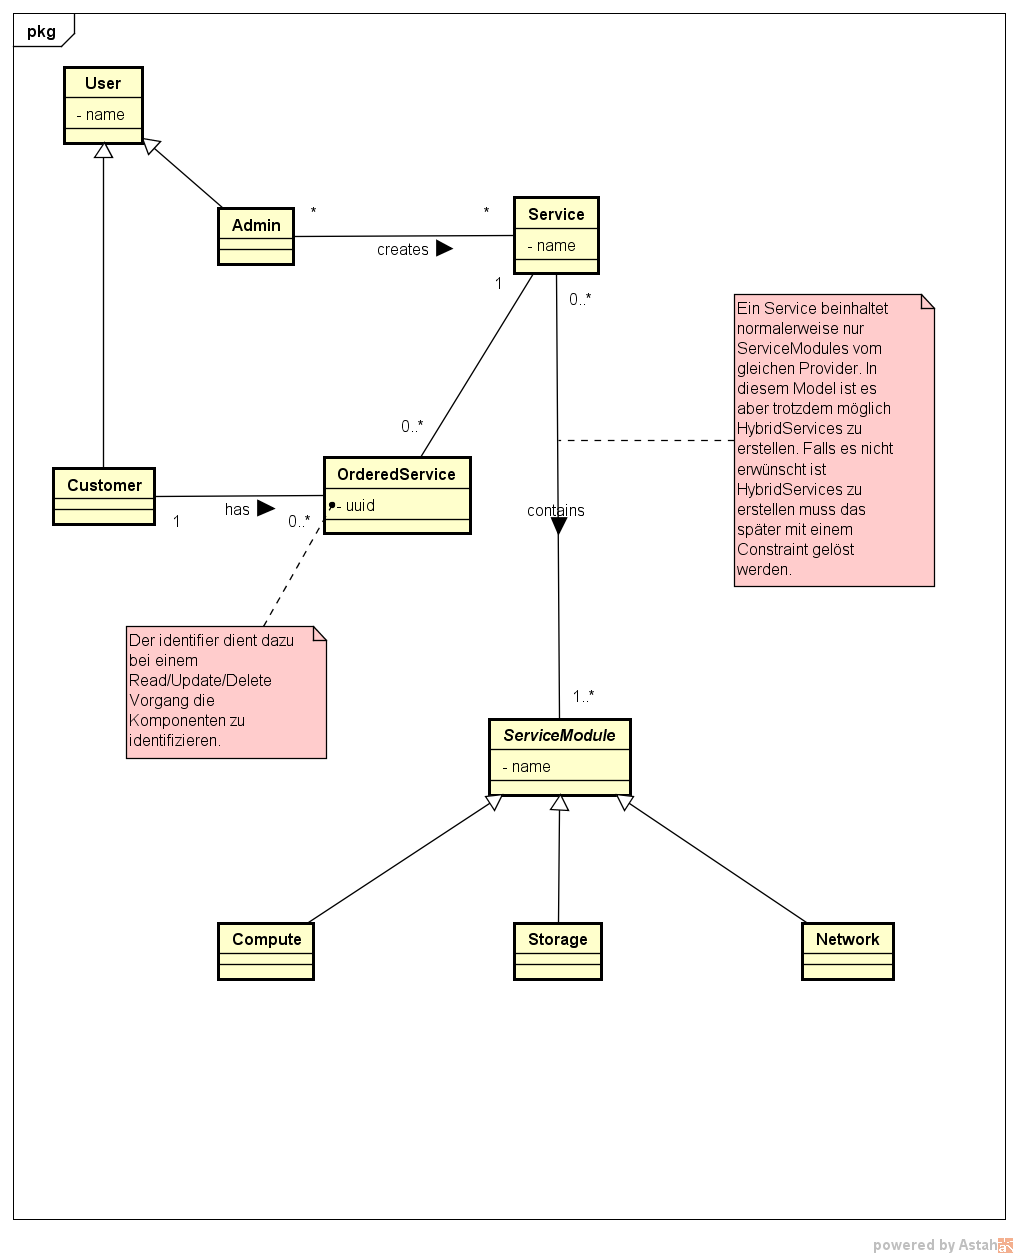
\includegraphics[width=\textwidth]{./03_Analyse/05_DomainModel/images/SDDC-DomainModel}
\caption{Domainmodell Skizze}
\end{figure}


%Anforderungen


%Design


%Appendix
\bibliographystyle{unsrt}
\bibliography{SDDC}
\end{document}
